\chapter{Mobile client}
\minitoc

\section{Lab Description}

\textit{The main objective of this assignment is to understand some of the some of the basic primitives and challenges of mobile computing.\\
You are required to expose Task manager’s Task entity as Google Endpoint (similar to the Todo item in the sample code) hosted on the Google App engine web application project, so that it can consumed by the mobile devises. Furthermore, also develop the functionality to send push notifications to the registered mobile devises whenever a new task is created on the app engine background. On the mobile application side, develop functionality for listing the tasks from the app engine background and also to display the push notification messages received from from the app engine backend whenever a new task is created on the app engine backend.}

\section{Solution}
The solution implemented makes use of the Android Development Tool Bundle; a collection of programs and tools assisting creation of software run on the Android platform. Using the Eclipe-integrated software suite the majority of the code needed to complete the assignment can be auto generated. During the development the Google plugin for Eclipse is also heavily used.\\
Communication between the parts of the distributed solution is handled by Google endpoints. These are java classes that exposes methods for receiving and modifying data objects. Each endpoint is expected to expose a single data entity, as defined by the javax.persistence namespace. The endpoint framework manages the communication between endpoints by converting method calls to REST requests and method return type to REST responses (see section \ref{rest_reflection}). Methods used by the endpoints are identified by use of method signature attributes defined in the com.google.api.server.spi.config namespace.\\
The solution consists of two eclipse projects: a backend and a client. The backend is deployed to the Google App Engine; a cloud service allowing for web services communicating via Google endpoints to be deployed and run on Googles dedicated servers. The client is an Android application communicating with the backend by use of Google endpoints.\\
In order to create the backend, a Task entity class is defined. This is a simple data object exposing the same data fields as the contents of task-manager-xml.xml. From this entity an endpoint exposing the entity can be generated. This endpoint provides functionality for receiving, adding, updating and deleting Tasks from the persistence managed by the service. Two additional endpoints are automatically set up to assists the program execution; one for transmitting device data, when a device registers for updates from the service, and one for sending and receiving message data. Persistence is managed by the framework, and accessed through the EntityManager class.\\
The Android clients control flow is entirely event driven. An application on this platform runs a number of activities, and these activities respond to events such as the screen being touched, or the device turning on and off. The application we create only run a single activity, RegisterActivity. This activity allows the user to register the device, so that it can receive notifications from the server. \\
We modify the TaskEndpoint class, so that insertion and updating of tasks triggers a broadcast message to all devices registered. The message contains a short list of the latest tasks to be added to the collection, printed out in a simple text format. We use a DeviceInfoEndpoint to gain access to the collection of devices that have registered to the service via RegisterActivity. We then simply iterate over this collection, and send the message to each device. In order to send the message we have to make use of the service´s API key; a unique number identifying the service on the Google App Engine. 


\section{Example Run}
In order to debug and run the client we are setting up a virtual Android machine that can execute the code.\\
A number of requests are send manually to the TaskEndpoint to create new Task objects on the server. Figure \ref{mobile_json_figure} shows the request to the server and the response. Consequently, a number of tasks are created on the site. Figure \ref{mobile_task_list_figure} shows a list of the tasks created.\\
\begin{figure}[ht]
	\centering
	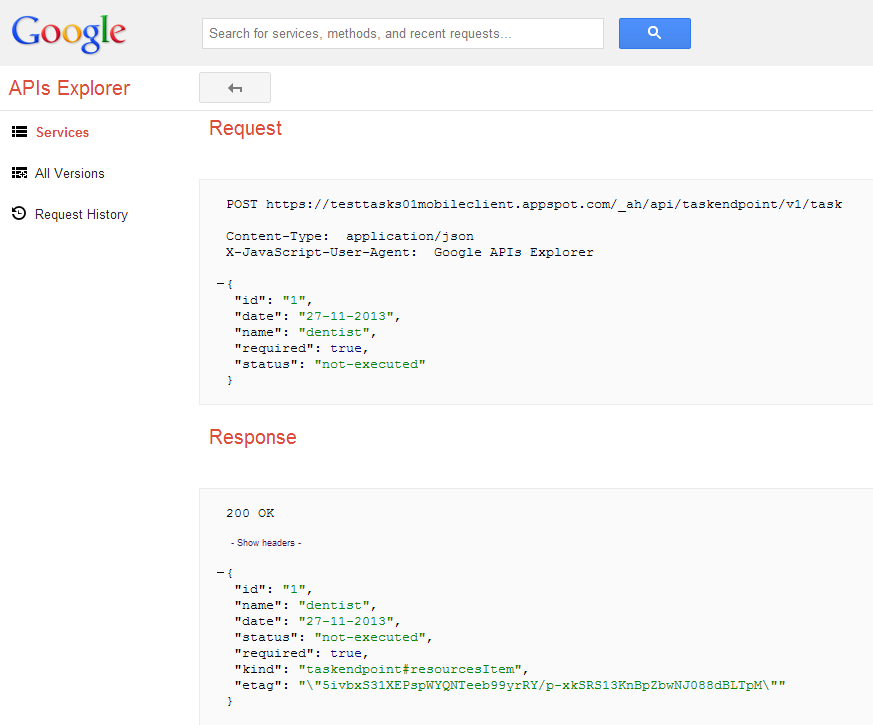
\includegraphics[scale=0.7]{images/googlecloud__createtask.png}
	\caption{creating a task}
	\label{mobile_json_figure}
\end{figure}
\begin{figure}[ht]
	\centering
	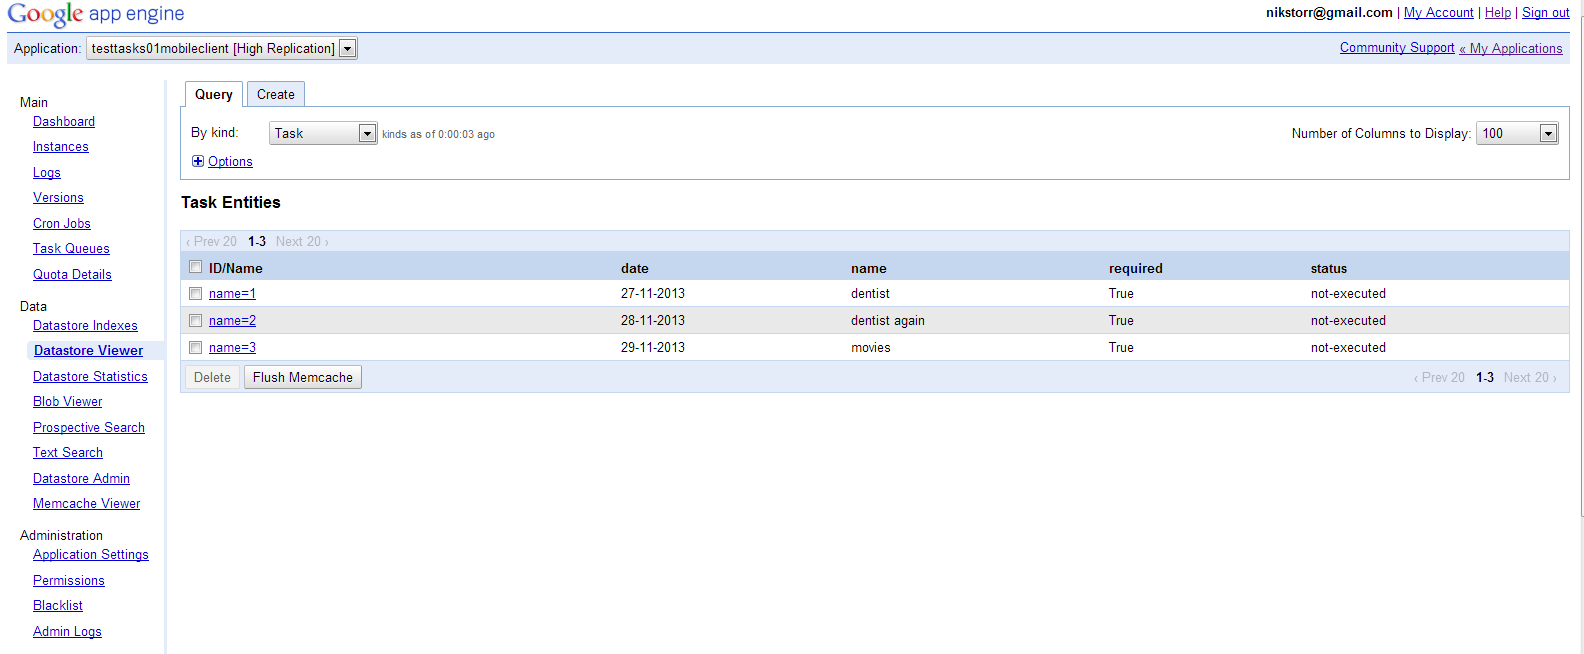
\includegraphics[scale=0.5]{images/googlecloud__taskexist.png}
	\caption{list of tasks created}
	\label{mobile_task_list_figure}
\end{figure}

The client is registered to receive updates whenever a new task is added to the Task collection. Figure \ref{mobile_registration_figure} shows the message informing that registration was successful.\\
\begin{figure}[ht]
	\centering
	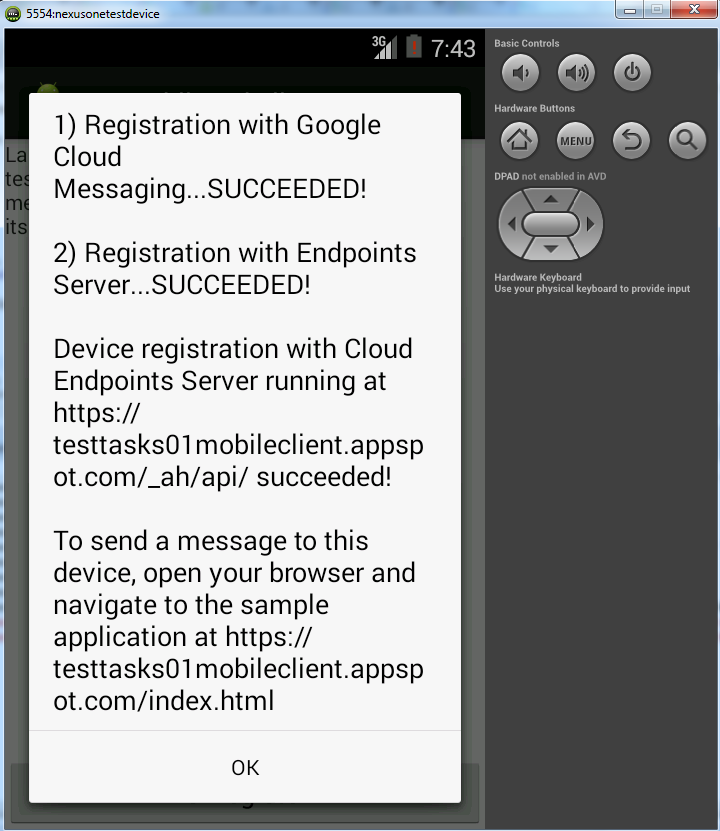
\includegraphics[scale=0.7]{images/googlemessagin_isonline_cloudmessaging.png}
	\caption{registration succeeds}
	\label{mobile_registration_figure}
\end{figure}

To test that communication happens properly a test message is sent manually. Figure \ref{mobile_message_figure} shows the message being sent at the server site, and figure \ref{mobile_hej_hej_hej_figure} shows the client receiving the message.\\
\begin{figure}[ht]
	\centering
	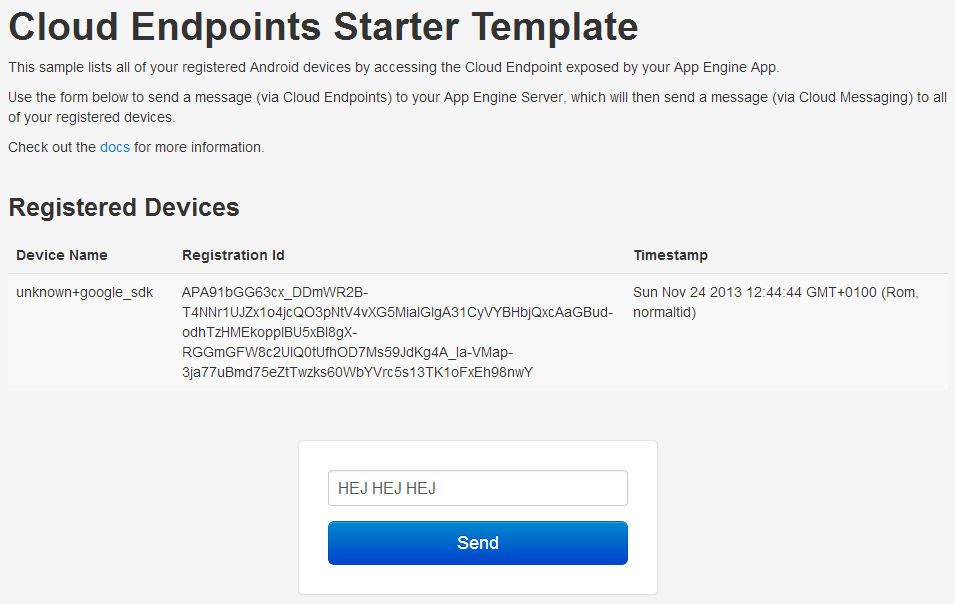
\includegraphics[scale=0.5]{images/googlemessagin_sendmessage.png}
	\caption{message being sent}
	\label{mobile_message_figure}
\end{figure}
\begin{figure}[ht]
	\centering
	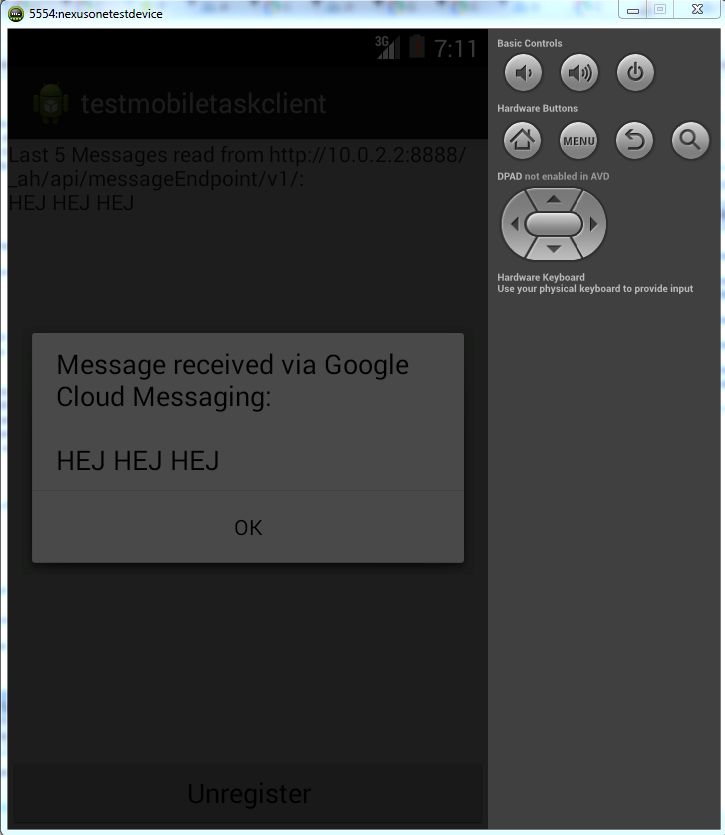
\includegraphics[scale=0.7]{images/googlecloudmessaging.png}
	\caption{message being received}
	\label{mobile_hej_hej_hej_figure}
\end{figure}

When a new Task is being created at the server site, the client receives the update message as shown in figure \ref{mobile_task_update_figure}.
\begin{figure}[ht]
	\centering
	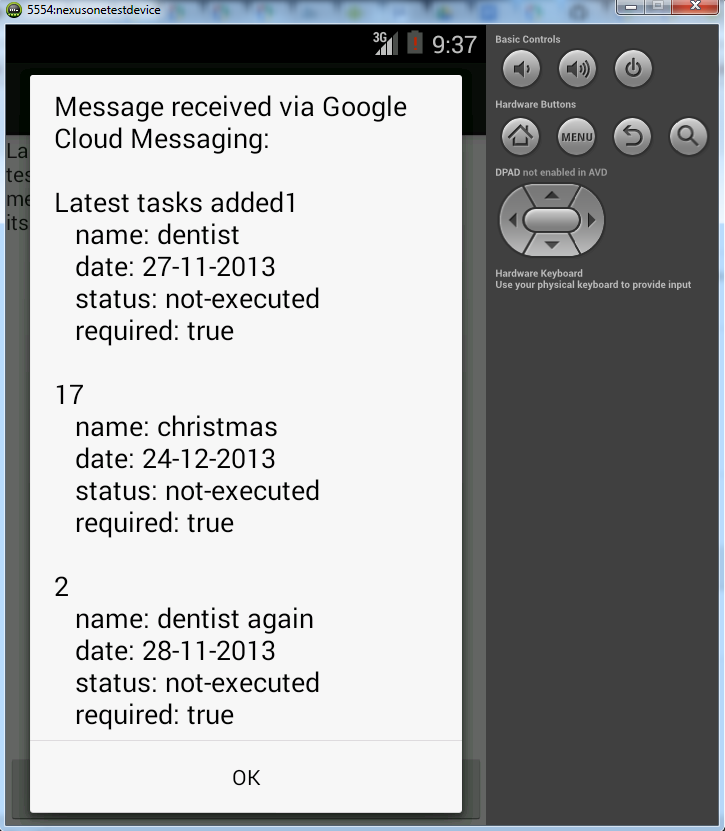
\includegraphics[scale=0.7]{images/googlecloud__tasksindevice.png}
	\caption{task update being received}
	\label{mobile_task_update_figure}
\end{figure}


\section{Reflection}

mobile applications are characterized first and foremost by volatility and instability. Volatility refers to connections that are assumed to fail more often than not, while instability refers to high-level formats and standards that are not expected to remain relevant to a given solution for an extended period of time. The Google endpoint technology used in the solution attempts to overcome the instability problem by relying on the well established and stable Http interface for communication, and thus centralizing definitions of data formats and protocols. \\
The volatility issue is never directly assessed in the exercise, as the mobile device involved is not a physical device but a simulation. Common solutions to volatile connections involves the device continuously scanning its surroundings for suitable connection providers, and preparing to switch between providers frequently and easily.\\
The Android client designed exemplifies several characteristics of the Android architecture:
\begin{itemize}
	\item The platform does not require compilation to a common code format, but supports embedding of other code languages, here among java. This could allow for a mobile application to be designed for several mobile platforms at once, without having to deal with a lot of platform-specific code.
	\item The system is entirely event driven. Activity objects are instantiated as an abstraction of running processes on the platform, and each activity listens for a number of relevant events, and reacts to them. No functional entry point (main method) exists for the application, only a designated main activity that is instantiated and started at program startup. In our specific solution the main activity only start a single activity; the register activity.
	\item The application switches between a number of states during execution. These include starting, running, pausing, restarting and stopping. The activities on the application reacts to these changes in state by listening to the relevant events.
\end{itemize}
In accordance with another problem common to mobile devices, namely limited memory, the Google App Engine manages all  object persistence in the solution. Given the data centred design of the task manager application, proper persistence performance can be expected to be a relevant characteristic.

\section{Conclusion}